% !TEX root = ../Micro.tex
\chapter{Nash Equilibrium and Subgame Perfection}

\section{Nash Equilibrium and Nash's Theorem}

\defn{Nash Equilibrium}{
  A strategy profile $\pr{\bar\sigma_1,\bar\sigma_2,\cdots,\bar\sigma_n}$ (where $\bar\sigma_i\in \Delta(S_i)$) is a Nash equilibrium of the game $G = \pr{S_i,u_i}_{i = 1}^n$ if for any player $i$,
  \[
  u_i(\bar\sigma_i,\bar\sigma_{-i})\ge u_i(s_i,\bar\sigma_{-i}),\quad \forall s_i\in S_i.
  \]
}

\rmkb[]{
  Equivalently we can define Nash equilibrium by
  \[
  u_i(\bar\sigma_i,\bar\sigma_{-i})\ge u_i(\sigma_i,\bar\sigma_{-i}),\quad \forall \sigma_i\in \Delta(S_i).
  \]
  But it suffices to only check pure strategies $s_i$ because mixed strategies are just probability distributions over pure strategies, and the expected utility of a mixed strategy is a convex combination of the utilities of the pure strategies.
}

\thmp{Nash}{
  Every finite game has a Nash equilibrium in mixed strategies.
}{
  Here we apply the Kakutani's Fixed Point Theorem.
  \thm{Kakutani's Fixed Point Theorem}{
    Suppose $F:X\rightrightarrows X$ (i.e., $F(x)\subseteq X$), and 
    \begin{itemize}
      \item $X$ is compact and convex;
      \item $F(x)$ is convex for all $x\in X$;
      \item $F$ has a closed graph, i.e., the set $\brace{(x,y)|y\in F(x)}$ is closed.
    \end{itemize}
    Then, there exists $x^*\in X$ such that $x^*\in F(x^*)$.
  }
  Let $X_i\equiv \Delta(S_i)$, and $X = X_1\times X_2\times \cdots \times X_n = \prod_{i = 1}^{n}\Delta(S_i)$. Define the best response correspondence $B_i:\prod_{j\ne i}\Delta(S_j) \rightrightarrows \Delta(S_i)$ by
  \[
  \sigma_i\in B_i(\sigma_{-i}) \iff u_i(\sigma_i,\sigma_{-i})\ge u_i(\sigma_i',\sigma_{-i}),\quad \forall \sigma_i'\in \Delta(S_i).
  \]
  And we define $B:X\rightrightarrows X$ by 
  \[
  B(\sigma) = \begin{pmatrix}
    B_1\\
    B_2\\
    \vdots\\
    B_n
  \end{pmatrix}(\sigma).
  \]
  It is easy to verify that $B(\sigma)$ is convex for all $\sigma\in X$, and $B$ has a closed graph. Therefore, by Kakutani's theorem, there exists $\bar\sigma\in X$ such that $\bar\sigma\in B(\bar\sigma)$, which means that $\bar\sigma$ is a Nash equilibrium.
}
\rmkb[]{
  \begin{itemize}
    \item ``Mixed strategies'' is important for Nash's Theorem. Finite games may not have NE in pure strategies.
    \item If $\bar\sigma$ is a NE, and $\bar\sigma_i(s_i)>0$, then $s_i$ must be a best response to $\bar\sigma_{-i}$, and thus $u_i(s_i,\bar\sigma_{-i})=u_i(\bar\sigma_i,\bar\sigma_{-i})$. In other words, if a pure strategy is played with positive probability in a mixed strategy NE (i.e., in the \textit{support} of the mixed strategy $\bar\sigma$), then it must yield the same expected payoff as the mixed strategy itself.
    \item Then why bother mixing? Because each player mixes to make other players mix. If a player chooses a pure strategy, then other players will have no incentive to mix, and thus the first player will have no incentive to mix either. Therefore, mixing can be a strategic move to induce other players to mix, which can lead to a more favorable outcome for the player.
  \end{itemize}
}

\section{Potential Games}

One of the central questions in game theory is whether a game has a \textit{pure strategy Nash equilibrium} (PSNE). Some games, like matching penny, have no PSNE. However, certain classes of games are guaranteed to have PSNE. Two important classes are:
\begin{itemize}
  \item Potential games
  \item Supermodular games
\end{itemize}

In this section we will focus on potential games, which are a broad class of games that include many interesting examples, such as congestion games, coordination games, and certain types of auctions. Potential games have a special structure that allows us to analyze them using a potential function, which captures the incentives of all players in a single function.

\subsection{Definition}

\defn{Potential Game}{
  A finite game $G = (S_i, u_i)_{i = 1}^n$ is called a \textit{potential game} if there exists a function $P: S \to \RR$ (where $S = S_1 \times S_2 \times \cdots \times S_n$) such that for every player $i$ and every pair of strategies $s_i, s_i' \in S_i$:
  \[
    u_i(s_i, s_{-i}) - u_i(s_i', s_{-i}) = P(s_i, s_{-i}) - P(s_i', s_{-i}),\quad s_{-i} \in S_{-i}.
  \]
  The function $P$ is called the \textit{potential function}.
}

\ex[Congestion Game]{
  Consider a road network where $n$ drivers choose routes. Let $s_i$ be the route chosen by driver $i$, $n_r(s)$ the number of drivers on route $r$ under profile $s$, and $c(r, k)$ the congestion cost incurred by each user of route $r$ when $k$ drivers use it. Driver $i$'s payoff is
  \[
    u_i(s_i, s_{-i}) = -c\!\bigl(s_i,\ n_{s_i}(s)\bigr).
  \]
  Define the potential function
  \[
    P(s) \;=\; -\sum_{r}\,\sum_{k=1}^{n_r(s)} c(r, k).
  \]
  When driver $i$ switches from route $r$ to route $r'$, the change in $P$ is exactly $c(r', n_{r'}(s) + 1) - c(r, n_{r}(s))$, which equals the change in driver $i$'s own payoff (up to sign). Hence $P$ is a potential function and the game admits a PSNE---the route assignment that minimizes total congestion cost.
}

\rmkb{
  \begin{itemize}
    \item Potential games can be thought of as games where all players have identical payoffs.
    \item Potential games arise naturally when:
\begin{itemize}
  \item Players care about a common objective (like aggregate welfare)
  \item Individual incentives are aligned with some global measure
  \item Strategic interactions are ``symmetric'' in the sense of cross-partial derivatives
\end{itemize}
    \item The potential function $P$ captures the payoff differences for individual players when they deviate from one strategy to another. The key insight is that a player's incentive to deviate depends only on how the potential function changes, not on the baseline payoff levels.
    \item In the continuous case with smooth payoff functions, a game is a potential game if and only if:

\[
  \begin{aligned}
    \frac{\partial P}{\partial s_i} = \frac{\partial u_i}{\partial s_i} \quad \text{for all players } i
  \end{aligned}
\]

This leads to the following necessary condition, for all pairs of players $i$ and $j$:
\[
  \frac{\partial^2 u_i}{\partial s_j \partial s_k} = \frac{\partial^2 u_j}{\partial s_k \partial s_j} \quad \text{whenever these derivatives exist.}
\]
  \end{itemize}
}

\subsection{Existence of PSNE in Potential Games}

\thmp{Existence of PSNE in Potential Games}{
  Every potential game has at least one pure strategy Nash equilibrium.
}{
  A PSNE of game $G$ is a maximizer of the potential function $P$. Since $S$ is finite (in the discrete case), $P$ attains its maximum. At such a maximum point $s^*$, if player $i$ deviates to any other strategy $s_i \neq s_i^*$, then:
\[
  u_i(s_i^*, s_{-i}^*) - u_i(s_i, s_{-i}^*) = P(s_i^*, s_{-i}^*) - P(s_i, s_{-i}^*) \geq 0
\]
Thus no player wants to deviate, so $s^*$ is a PSNE.
}

\rmkb[]{
Different information structures (simultaneous move vs. sequential move) can lead to different equilibria in general games. However, in potential games, the set of pure strategy Nash equilibria is often robust across different information structures. This is because the potential function captures the incentives of all players in a way that is independent of the timing of moves. As a result, the same strategy profiles that maximize the potential function will be equilibria regardless of whether players move simultaneously or sequentially.
}

\section{Supermodular Games}

While potential games ensure the existence of PSNE through a global potential function, supermodular games approach the problem differently: they rely on the structure of strategic complementarities between players' actions.

The key insight is \textit{strategic complementarity}: if one player's action increases, it becomes more attractive for other players to increase their actions as well. This creates a natural coordination mechanism that leads to equilibrium. Unlike potential games, which require a global objective function, supermodular games only require local complementarity conditions on payoffs.

Examples of strategic complementarity abound:
\begin{itemize}
  \item In a price competition setting, if a competitor raises prices, your prices become more attractive to consumers, so you want to raise your price too.
  \item In technology adoption, if more people adopt a technology, the benefits of adoption increase for you (network effects).
  \item In public goods games, if others contribute more, your optimal contribution may also increase.
\end{itemize}

\subsection{Definitions}

We need lattice-theoretic concepts to formalize strategic complementarity. 

\defn{Meet \& Join}{
  Let $x$ and $y$ be two vectors of $\RR^n$. The \textit{meet} of $x$ and $y$, denoted by $x\meet y$, is the coordinate-wise minimum:
  \[
    x\meet y = \begin{pmatrix}
      \min(x_1,y_1)\\
      \min(x_2,y_2)\\
      \vdots\\
      \min(x_n,y_n)\\
    \end{pmatrix}
    \]
    The \textit{join} of $x$ and $y$, denoted by $x\join y$, is the coordinate-wise maximum:
    \[
    x\join y = \begin{pmatrix}
      \max(x_1,y_1)\\
      \max(x_2,y_2)\\
      \vdots\\
      \max(x_n,y_n)\\
    \end{pmatrix}
    \]
}

\rmkb{
  Meet and join decompose a pair of strategy profiles into their ``lower bound'' and ``upper bound'' in each dimension. Later we will see, if a payoff function is supermodular, then being at both extremes (the largest and smallest actions) together is at least as good as being at the two middle ground positions.
}

\defn{Supermodular Function}{
  A function $f: \RR^n \to \RR$ is \textit{supermodular} if for all $x, y \in \RR^n$:
  \[
    f(x\meet y) + f(x\join y) \geq f(x) + f(y)
  \]
  This is called the \textit{supermodularity inequality}.
}

Intuitively, the supermodularity inequality says: having some coordinates large and others small is better than having all coordinates at intermediate levels.

In a game setting, we say player $i$'s payoff is supermodular if:
\[
  u_i(s) + u_i(s') \leq u_i(s \meet s') + u_i(s \join s') \quad \forall s, s' \in S
\]

This means: player $i$'s payoff is supermodular in their own strategy relative to opponents' strategies.

\rmkb[]{
  When $f$ is twice continuously differentiable, supermodularity is equivalent to:

\[
  \frac{\partial^2 f}{\partial x_i \partial x_j} \geq 0 \quad \text{for all } i \neq j.
\]
This means: if you increase $x_i$, the marginal benefit of increasing $x_j$ also increases (\textit{strategic complementarity}).
}



\subsection{Existence of PSNE in Supermodular Games}

The next two lemmas establish that best response correspondences have monotonicity properties under supermodularity, which enables us to use fixed point theorems.

\lemp{Monotonicity of Best Responses}{
  Suppose $u:[0,1]^p \times [0,1]^q \to \RR$ is supermodular. Suppose $y', y'' \in [0,1]^q$ with $y'' \geq y'$. Let $x' \in [0,1]^p$ be a maximizer of $u(\cdot, y')$, and $x'' \in [0,1]^p$ be a maximizer of $u(\cdot, y'')$. Then $x' \meet x''$ is a maximizer of $u(\cdot, y')$, and $x' \join x''$ is a maximizer of $u(\cdot, y'')$.
}{
  By construction, since $x'$ maximizes $u(\cdot, y')$ and $x''$ maximizes $u(\cdot, y'')$:
  \[
    u(x', y') \geq u(x' \meet x'', y')
  \]
  
  Also note that $u(x' \meet x'', y') = u(x' \meet x'', y' \meet y'')$ since $y' \meet y'' = y'$ (as $y' \leq y''$).
  
  Similarly:
  \[
    u(x'', y'') \geq u(x' \join x'', y'') = u(x' \join x'', y' \join y'')
  \]
  
  By supermodularity:
  \[
    u(x', y') + u(x'', y'') \geq u(x' \meet x'', y' \meet y'') + u(x' \join x'', y' \join y'')
  \]
  
  Suppose $u(x', y') > u(x' \meet x'', y' \meet y'')$. Then:
  \[
    u(x', y') + u(x'', y'') > u(x' \meet x'', y' \meet y'') + u(x' \join x'', y' \join y'')
  \]
  which violates supermodularity.
  
  Therefore, we must have:
  \[
    \begin{aligned}
      u(x', y') & = u(x' \meet x'', y' \meet y'')\\
    u(x'', y'') & = u(x' \join x'', y' \join y'')
    \end{aligned}
  \]
  
  This means both $x' \meet x''$ and $x' \join x''$ are maximizers at the respective points.
}

\lemp{Monotonicity of Largest Maximizers}{
  Suppose $u:[0,1]^p \times [0,1]^q \to \RR$ is supermodular. Define:
  \[
    h(y) = \max\{x : x \text{ maximizes } u(\cdot, y)\}
  \]
  (the largest maximizer). Then $h$ is non-decreasing: if $y'' \geq y'$, then $h(y'') \geq h(y')$.
}{
  Suppose $y'' \geq y'$. Let $x' = h(y')$ and $x'' = h(y'')$ be the largest maximizers at $y'$ and $y''$ respectively. By the previous lemma, $x' \meet x''$ maximizes $u(\cdot, y')$ and $x' \join x''$ maximizes $u(\cdot, y'')$.
  
  Since $x'\join x''$ is a maximizer at $y''$ and $x''$ is the largest maximizer at $y''$, we have $x'' \geq x' \join x''$. By definition, $x'\join x'' \geq x'$. So $x'' \geq x'$. Therefore, $h(y'') = x'' \geq x' = h(y')$.
}

\thmp{Existence of PSNE in Supermodular Games}{
  Every finite supermodular game has at least one pure strategy Nash equilibrium.
}{
This is a direct result of Tarski's Fixed Point Theorem.

  \thm{Tarski's Fixed Point Theorem}{If $f: L \to L$ is a non-decreasing function on a complete lattice $L$, then $f$ has a fixed point.}

  \rmk{
    \emph{Why Tarski holds (sketch).} Let $L$ be a complete lattice with top $\top$ and bottom $\bot$. The set $A = \{x \in L : x \le f(x)\}$ contains $\bot$ (since $\bot \le f(\bot)$) and is therefore non-empty. Let $\bar x = \sup A$, which exists by completeness. Monotonicity gives $f(x) \le f(\bar x)$ for every $x \in A$, and combining with $x \le f(x)$ yields $x \le f(\bar x)$, so $f(\bar x)$ is an upper bound of $A$ and hence $\bar x \le f(\bar x)$. Applying $f$ once more and using monotonicity, $f(\bar x) \le f(f(\bar x))$, so $f(\bar x) \in A$ and $f(\bar x) \le \bar x$. Together: $f(\bar x) = \bar x$. The argument is constructive on finite lattices: iterate $f$ on $\bot$ until the sequence stabilizes.
  }

  For each player $i$, define $b_i(s_{-i})$ as the largest maximizer of $u_i(\cdot, s_{-i})$. By the lemmas above, $b_i$ is non-decreasing in $s_{-i}$.
  
  Define the best response mapping $b: S \to S$ by:
  \[
    b(s) = (b_1(s_{-1}), b_2(s_{-2}), \ldots, b_n(s_{-n}))
  \]
  
  Since $b$ is component-wise non-decreasing and $S$ is a finite lattice, by \textit{Tarski's Fixed Point Theorem}, $b$ has a fixed point $\bar{s}$, i.e., $b(\bar{s}) = \bar{s}$. This fixed point is a Nash equilibrium.
}

\ex[Bertrand Duopoly with Differentiated Products]{
  Consider two firms competing in prices. Let $D_i(p_1, p_2)$ be firm $i$'s demand, which is decreasing in its own price $p_i$ and increasing in the competitor's price $p_j$. With constant marginal cost $c$, firm $i$'s profit is:
  \[
    \pi_i(p_1, p_2) = (p_i - c) D_i(p_1, p_2)
  \]
  
  The key observation is:
  \[
    \frac{\partial^2 \pi_i}{\partial p_i \partial p_j} = \frac{\partial}{\partial p_j}\left[\frac{\partial \pi_i}{\partial p_i}\right] > 0
  \]
  
  This is because when the competitor's price increases, the marginal profit from raising your own price increases (since demand becomes more favorable). Thus, firm $i$'s profit is supermodular in $(p_1, p_2)$, and the duopoly game has a PSNE.
}

\section{Subgame Perfect Nash Equilibrium}

Nash equilibrium constrains only on-path play. In extensive-form games---where players move sequentially and can condition on what they have observed---this is too weak: many Nash equilibria are sustained by threats that the threatener would never actually carry out. Subgame perfection refines NE by demanding optimality in every \emph{subgame}, ruling out such non-credible threats.

\subsection{Definitions and Existence}

\defn{Subgame}{
  Given an extensive form $T$, a subgame $T'$ is some node $r\in T$ and all its succeeding nodes such that if an information set $I$ intersects $T'$, then all nodes in $I$ are also in $T'$.
}

\defn{Subgame Perfect Nash Equilibrium}{
  $\sigma$ is a \textit{subgame perfect equilibrium} if
  \begin{itemize}
    \item $\sigma$ is a Nash equilibrium.
    \item $\sigma$ induces a Nash equilibrium in every subgame $T'\subseteq T$.
  \end{itemize}
}

\ex[Entry Deterrence Game]{Consider the following game:
\begin{center}
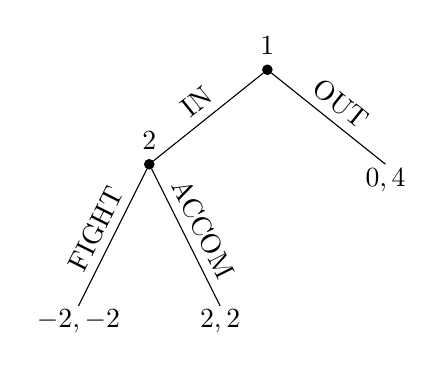
\begin{tikzpicture}[scale=1]
    % Node styles
    \tikzset{solid node/.style={circle,draw,fill=black,inner sep=1.2pt}}

    % --- Level 0: Root (Player 1) ---
    \node[solid node, label=above:1] (root) at (0,0) {};

    % --- Level 1 (Player 1's choices) ---
    \node[solid node, label=above:2] (n2_left) at (-1.5, -1.2) {};
    \coordinate (out) at (1.5, -1.2);

    % Edges from Root
    \draw (root) -- (n2_left) node[midway, above, sloped] {IN};
    \draw (root) -- (out) node[midway, above, sloped] {OUT};

    % --- Level 2: Terminal nodes (Player 2's choices lead here) ---
    \coordinate (fight) at (-2.4, -3);
    \coordinate (accom) at (-0.6, -3);

    % Edges from Player 2
    \draw (n2_left) -- (fight) node[midway, above, sloped] {FIGHT};
    \draw (n2_left) -- (accom) node[midway, above, sloped] {ACCOM};

    % --- Payoffs ---
    \node at (1.5, -1.4) {$0, 4$};
    \node at (-2.4, -3.2) {$-2, -2$};
    \node at (-0.6, -3.2) {$2, 2$};
\end{tikzpicture}
\end{center}

From its normal form (payoff matrix) below, we know that there are two Nash equilibria: (OUT, FIGHT) and (IN, ACCOM).

\[
\begin{array}{c|cc}
 & \text{FIGHT} & \text{ACCOM} \\
\hline
\text{OUT} & 0, 5 & 0, 5 \\
\text{IN} & -2, -2 & 2, 2
\end{array}
\]

However, only (IN, ACCOM) is a subgame perfect equilibrium, because if Player 1 chooses IN, then Player 2's best response is to choose ACCOM (so to choose FIGHT is not a credible threat). Therefore, the unique subgame perfect equilibrium is (IN, ACCOM).

Suppose now the game is repeatedly played for $T = 20$ times.
At $t = 1$, Player 1 chooses IN or OUT. If Player 1 chooses OUT, the game ends. If Player 1 chooses IN, then in any period $t\ge 1$, the Player 1 can choose to stay (IN) or exit (OUT). If OUT is ever chosen by Player 1, then OUT for all the periods onwards.

Clearly, using backward induction, we know that the unique subgame perfect equilibrium is for Player 1 to choose IN and Player 2 to choose ACCOM in all periods.

However, if we add one additional constraint: Player 1 can only fight for at most 15 periods, then the analysis changes.

\clmp{}{
  The unique SPE with the constraint is that
  \begin{itemize}
    \item Player 1 never enters (IN), and
    \item Player 2 chooses FIGHT if Player 1 chooses IN.
  \end{itemize}
}{
  Suppose that Player 1 has entered and been fought for the previous 14 periods. In period $t=15$, if Player 1 chooses IN, Player 2 compares the payoffs of FIGHT and ACCOM:
  \begin{itemize}
    \item If Player 2 chooses \text{FIGHT}: Player 1's capacity is exhausted, forcing them to choose OUT from $t=16$ to $t=20$. Player 2's total remaining payoff is $-2 (\text{at } t=15) + 5 \times 4 (\text{monopoly profit}) = 18$.
    \item If Player 2 chooses \text{ACCOM}: Player 1 stays in the market. Player 2's total remaining payoff is $2 (\text{at } t=15) + 5 \times 2 (\text{duopoly profit}) = 12$.
  \end{itemize}
  Since $18 > 12$, FIGHT becomes a \textit{credible threat} at $t=15$. Anticipating this, Player 1 will choose OUT at $t=15$ to avoid the $-2$ payoff.

  Consider period $t=14$. Player 1 anticipates that choosing IN will result in Player 2 choosing FIGHT (to trigger the exit at $t=15$ and secure future monopoly profits). Choosing IN at $t=14$ followed by exit at $t=15$ yields a lower payoff than choosing OUT immediately at $t=14$.

  Following this logic backward to $t=1$, consequently, the only rational choice for Player 1 is to never enter (OUT), and for Player 2 to threaten to FIGHT at any entry node.
}

}

\thmp{}{
  Every finite game in extensive form has at least one subgame perfect equilibrium.
}{
The proof is to find all subgames that do not have any proper subgames. In each such subgame, find a Nash equilibrium of the subgame, and replace each node by expected payoffs from any Nash equilibrium of the subgame.
}

\rmkb[]{
The notion of subgame perfect equilibrium is to generalize backward induction to games with imperfect information.
}

\subsection{The Backward Induction Algorithm}

The proof of the existence theorem is constructive: it gives an explicit \emph{algorithm} for computing an SPE in any finite extensive-form game. The procedure---\textbf{backward induction}---is the workhorse of finite-horizon analysis.

\state{Backward Induction Algorithm}{
  Let $T$ be a finite extensive-form game.
  \begin{enumerate}
    \item \textbf{Identify minimal subgames.} A subgame is \emph{minimal} if it contains no proper subgame. Equivalently, every information set inside it is a singleton in which only one player moves before reaching a terminal node.
    \item \textbf{Solve each minimal subgame.} Find a Nash equilibrium of the minimal subgame (in finite games this exists, by Nash's theorem applied to the subgame's normal form).
    \item \textbf{Substitute continuation payoffs.} Replace every minimal subgame by a single terminal node carrying the equilibrium payoff vector. This yields a smaller extensive-form game $T'$ with one less ``layer.''
    \item \textbf{Recurse.} Apply Steps 1--3 to $T'$. Terminate when only the root remains; the strategies recorded along the way constitute an SPE.
  \end{enumerate}
}

\rmkb[Why Backward Induction Produces an SPE]{
  By construction, the strategies prescribed in each minimal subgame are a Nash equilibrium of that subgame. After substitution, the next iteration treats those subgames as terminal nodes with fixed payoffs, so any Nash equilibrium of the reduced game $T'$ remains a Nash equilibrium when expanded back. Iterating, the prescribed strategies form a Nash equilibrium in every subgame---which is exactly the SPE condition. The argument is the game-theoretic analogue of \textbf{dynamic programming}: a globally optimal plan is built by stitching together locally optimal continuations.
}

\rmkb[Verification via the One-Deviation Property]{
  A practical corollary: to check that a candidate strategy profile $\sigma^*$ is an SPE, it suffices to verify, at every history (or every information set in the perfect-information case), that no player can profitably deviate by changing her action at that single node and reverting to $\sigma^*$ thereafter. This is the \textbf{one-shot deviation principle}, a finite-horizon analogue of the result we will state and prove for infinitely repeated games in the chapter on dynamic games. The principle reduces SPE verification from a global check across all alternative strategies to a local, period-by-period inequality at each node---precisely what the entry-deterrence example above (with Player 1's 15-period capacity constraint) implicitly relied on.
}

The backward-induction algorithm settles existence and provides a constructive solution method, but it does \emph{not} guarantee uniqueness: if a minimal subgame has multiple Nash equilibria, choosing different ones leads to different SPEs. This multiplicity is what powers the finite-horizon Folk Theorem (in the chapter on dynamic games): when a stage game has several payoff-distinct NE, the choice of which NE to play in late periods can be used as a reward or punishment to sustain non-NE play in early periods.

\ex[Centipede Game]{

\begin{center}
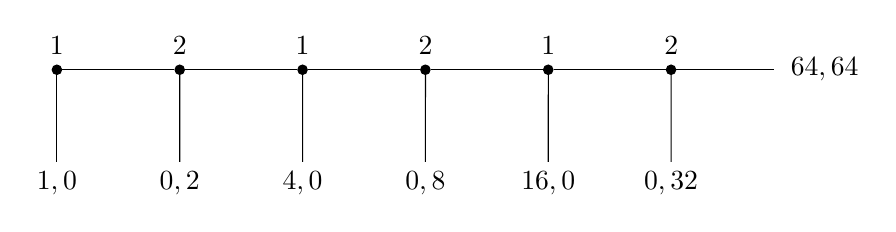
\begin{tikzpicture}[scale=1.3, font=\normalsize]
    \tikzset{solid node/.style={circle,draw,fill=black,inner sep=1.2pt}}

    % Main horizontal chain of nodes (closer spacing)
    \node[solid node, label=above:1] (p1_1) at (0, 0) {};
    \node[solid node, label=above:2] (p2_1) at (1.2, 0) {};
    \node[solid node, label=above:1] (p1_2) at (2.4, 0) {};
    \node[solid node, label=above:2] (p2_2) at (3.6, 0) {};
    \node[solid node, label=above:1] (p1_3) at (4.8, 0) {};
    \node[solid node, label=above:2] (p2_3) at (6, 0) {};
    \coordinate (end) at (7, 0) {};

    % Horizontal chain edges (no labels)
    \draw (p1_1) -- (p2_1);
    \draw (p2_1) -- (p1_2);
    \draw (p1_2) -- (p2_2);
    \draw (p2_2) -- (p1_3);
    \draw (p1_3) -- (p2_3);
    \draw (p2_3) -- (end);

    % Downward branches (Exit payoffs, shorter)
    \draw (p1_1) -- (0, -0.9) node[below] {$1,0$};
    \draw (p2_1) -- (1.2, -0.9) node[below] {$0,2$};
    \draw (p1_2) -- (2.4, -0.9) node[below] {$4,0$};
    \draw (p2_2) -- (3.6, -0.9) node[below] {$0,8$};
    \draw (p1_3) -- (4.8, -0.9) node[below] {$16,0$};
    \draw (p2_3) -- (6, -0.9) node[below] {$0,32$};

    % Final outcome (on the right)
    \node at (7.5, 0) {$64,64$};

\end{tikzpicture}
\end{center}

    The unique subgame perfect equilibrium is for each player to exit immediately at their first decision node, yielding payoff $(1, 0)$. However, the backward induction outcome $(1, 0)$ is Pareto dominated by the outcome $(64, 64)$ at the end. Both players would be better off if the game continued to the end, but the equilibrium logic prevents this.
}

\subsection{Trembling-Hand Perfect Equilibrium}

\ex[Selten's Horse]{

\begin{center}
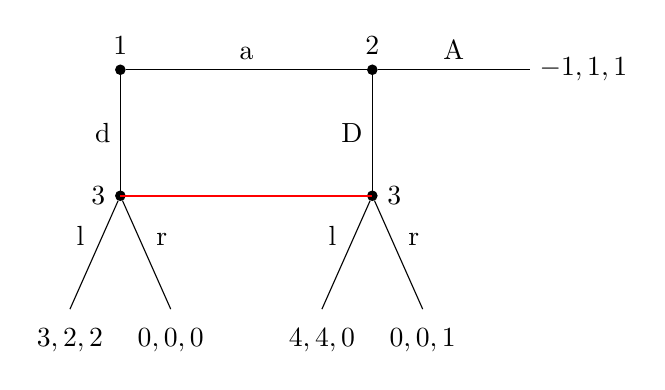
\begin{tikzpicture}[scale=0.8, font=\normalsize]
    \tikzset{solid node/.style={circle,draw,fill=black,inner sep=1.2pt}}

    % Level 0 - Player 1 (moved up, was p2_left)
    \node[solid node, label=above:1] (p1) at (-2, 0) {};

    % Level 0 - Player 2 (was p2_right)
    \node[solid node, label=above:2] (p2) at (2, 0) {};

    % Tree trunk connecting Player 1 and Player 2
    \draw (p1) -- (p2) node[midway, above] {a};

    % Level 1 - Player 3 nodes (with information set dashed line)
    \node[solid node, label=left:3] (p3_left) at (-2, -2) {};
    \node[solid node, label=right:3] (p3_right) at (2, -2) {};

    % Edges from Player 1 to left Player 3
    \draw (p1) -- (p3_left) node[midway, left] {d};

    % Edges from Player 2 to right Player 3
    \draw (p2) -- (p3_right) node[midway, left] {D};

    % Information set: red solid line connecting the two player 3 nodes
    \draw[red, thick] (-2, -2) -- (2, -2);

    % Branch from Player 2 going right to outcome
    \draw (p2) -- (4.5, 0) node[midway, above] {A} node[right] {$-1,1,1$};

    % Level 2 - Terminal outcomes from left Player 3
    \draw (p3_left) -- (-2.8, -3.8) node[midway, above left] {l};
    \node at (-2.8, -4.3) {$3,2,2$};

    \draw (p3_left) -- (-1.2, -3.8) node[midway, above right] {r};
    \node at (-1.2, -4.3) {$0,0,0$};

    % Level 2 - Terminal outcomes from right Player 3
    \draw (p3_right) -- (1.2, -3.8) node[midway, above left] {l};
    \node at (1.2, -4.3) {$4,4,0$};

    \draw (p3_right) -- (2.8, -3.8) node[midway, above right] {r};
    \node at (2.8, -4.3) {$0,0,1$};

\end{tikzpicture}
\end{center}

There are two pure strategy Nash equilibria: $(d, A, l)$ and $(a, A, r)$. Since this game has no proper subgames, both equilibria are subgame perfect.

However, the SPE $(d, A, l)$ appears problematic: if Player 1 accidentally chooses $a$ instead of $d$, Player 2 would prefer to choose $D$ rather than $A$. This suggests the equilibrium is not robust to small mistakes.
}

Recall that $\sigma$ is a Nash equilibrium if and only if for each player $i$ and any pure strategy $s_i'$: $u_i(\sigma_i,\sigma_{-i}) \geq u_i(s_i',\sigma_{-i})$, and for all the pure strategies that are in the support of $\sigma_i$, the expected payoff is the same: $u_i(s_i,\sigma_{-i}) = u_i(\sigma_i,\sigma_{-i})$ for all $s_i$ such that $\sigma_i(s_i) > 0$.
Hence, if for some pure strategy $s_i'$, we have $u_i(\sigma_i,\sigma_{-i}) > u_i(s_i',\sigma_{-i})$, then $\sigma_i(s_i') = 0$.

To formalize the intuition from the previous example of Selten's Horse, suppose all players' choices are subject to small trembles (mistakes).

\defn{$\varepsilon$-Equilibrium}{
  A mixed strategy profile $\sigma^{\varepsilon}$ is an \textit{$\varepsilon$-equilibrium} (for small $\varepsilon > 0$) if:
  \begin{itemize}
    \item Every pure strategy has positive probability: $\sigma_i^{\varepsilon}(s_i) > 0$ for all $i$ and $s_i$.
    \item Strategies that are not a best response are played with low probability: if $u_i(s_i',\sigma_{-i}^{\varepsilon}) > u_i(s_i,\sigma_{-i}^{\varepsilon})$, then $\sigma_i^{\varepsilon}(s_i') < \varepsilon$.
  \end{itemize}
}

\defn{Trembling Hand Perfect Equilibrium}{
  A strategy profile $\sigma$ is a \textit{trembling hand perfect equilibrium} (THPE) if it is the limit of a sequence of $\varepsilon$-equilibria $\sigma^{\varepsilon}$ as $\varepsilon \to 0$.
}
